\section{Statistika}

\begin{frame}
    \sectionpage
\end{frame}

\begin{frame}
    \tableofcontents[currentsection, hideothersubsections]
\end{frame}


    \subsection{Osnovni pojmi statistike}

        \begin{frame}
            \frametitle{Osnovni pojmi statistike}

            \begin{alertblock}{}
                \textbf{Populacija} je množica, ki jo statistično proučujemo. 
                Element populacije imenujemo \textbf{statistična enota}. 
            \end{alertblock}
            
            \begin{alertblock}{}
                \textbf{Vzorec} je podmnožica populacije, katere elementi predstavljajo največjo možno mero značilnosti celotne množice. 
                Vzorec izberemo, kadar je celotna populacija prevelika množica, da bi analizirali vse njene elemente. \\
                
                \begin{itemize}
                    \item \textbf{Reprezentativen vzorec} je vzorec, ki je izbran tako, da predstavlja značilnosti celotne populacije.
                    \item \textbf{Slučajni vzorec} je vzorec, ki je izbran naključno -- vsi elementi populacije imajo enako možnost, da bodo izbrani.
                \end{itemize}

                \textbf{Numerus} je število elementov vzorca. Oznaka $N$. 
            \end{alertblock}

        \end{frame}    


        \begin{frame}
            \begin{alertblock}{}
                \textbf{Statistična spremenljivka/podatek/znak} je vrednost ali lastnost, ki jo proučujemo.
            \end{alertblock}

            \begin{alertblock}{Vrste statističnih spremenljivk}
                \begin{itemize}
                    \item \textbf{opisne/kvalitativne} statistične spremenljivke
                    \item \textbf{vrstne/ordinalne} statistične spremenljivke
                    \item \textbf{številske/kvantitivne} statistične spremenljivke
                \end{itemize}
                
            \end{alertblock}

            \begin{block}{Številske statistične spremenljivke}
                \begin{itemize}
                    \item \textbf{diskretne} številske spremenljivke -- zavzamejo lahko posamezne vrednosti
                    \item \textbf{zvezne} številske spremenljivke -- zavzamejo lahko vsako vrednost z nekega intervala
                \end{itemize}

            \end{block}


        \end{frame}


        %%%% naloge

        \begin{frame}
            \only<2->{\begin{exampleblock}{Naloga}
                Zapišite, kaj je v danem primeru populacija, vzorec, statistična enota, spremenljivka in 
                ugotovite ali je spremenljivka opisna ali numerična in, če je numerična, ugotovite, ali je zvezna ali diskretna.
                \only<3->{\begin{itemize}
                        \item Na spletni strani je anketa z vprašanjem ``Ali imate doma pomivalni stroj?''. Nanjo je odgovorilo $254$ ljudi. 
                        \item V televizijski oddaji gledalci glasujejo za dva kandidata. 
                        \item Razrednik svojih $28$ dijakov vpraša, kolikšna je oddaljenost njihovega doma do šole.
                        \item Maturant piše seminarsko nalogo z naslovom ``Uporaba TikTok-a med srednješolci''. Pridobil je odgovore $369$ srednješolcev, ki so odgovarjali na vprašanje ``Ali~uporabljaš~TikTok?'' 
                        \item Znanstveniki pri raziskavi spremljajo, koliko jajc znesejo kokoši na slovenskih farmah na mesec.
                \end{itemize}}
            \end{exampleblock}}
        \end{frame}

        \begin{frame}

                \begin{columns}
                    \column{0.45\textwidth}


            \only<2->{\begin{exampleblock}{Naloga}
                    Slovenija ima več kot $6000$ naselij. Statistični urad Republike Slovenije je januarja 2024 naredil analizo naselij glede na število prebivalcev. 
                    Rezultati so prikazani v tabeli. \\~
                    
                    \only<4->{Zapišite, kaj je v danem primeru populacija, statistična enota, spremenljivka in ugotovite ali je spremenljivka opisna ali numerična in, 
                    če je numerična, ugotovite ali je zvezna ali diskretna.}
            \end{exampleblock}}

                    \column{0.5\textwidth}
                    \only<3->{\begin{table}
                        \centering
                        \begin{tabular}{||c|c||} 
                        \hhline{|t:==:t|}
                        \rowcolor[rgb]{0.843,0.718,0.718} 
                        velikostni razred naselja  & število naselij   \\ 
                        \hhline{|:==:|}
                        $0$ & $57$    \\ 
                        \hline
                        $1-24$ & $719$    \\ 
                        \hline
                        $25-49$ & $851$    \\ 
                        \hline
                        $50-99$ & $1256$     \\
                        \hline
                        $100-199$ & $1444$     \\
                        \hline
                        $200-499$ & $1109$     \\
                        \hline
                        $500-999$ & $359$     \\
                        \hline
                        $1000-4999$ & $199$     \\
                        \hline
                        $5000-9999$ & $23$     \\
                        \hline
                        $10000-49999$ & $16$     \\                    
                        \hline
                        $50000+$ & $2$     \\
                        \hhline{|b:==:b|}
                        \end{tabular}
                    \end{table}}
                \end{columns}
                
        \end{frame}



    \subsection{Urejanje in grupiranje podatkov}

        \begin{frame}
            \frametitle{Urejanje in grupiranje podatkov}

            \begin{block}{}
                Podatke, pridobljene v posamezni raziskavi, moramo najprej urediti. \\
                Če podatkov ni veliko, jih uredimo po velikosti v \textbf{ranžirno vrsto}, sicer jih združujemo v skupine, \textbf{frekvenčne razrede}.
            \end{block}

            \begin{block}{}
                Podatek z največjo vrednostjo označimo z $x_{max}$, podatek z najnižjo vrednostjo pa $x_{min}$.
            \end{block}

            \begin{alertblock}{}
                \textbf{Frekvenca} $f$ statističnega znaka je posamezno število diskretnih statističnih enot iste vrednosti.
            \end{alertblock}

            \begin{alertblock}{}
                \textbf{Frekvenčni razred} je skupina podatkov iz vzorca. Frekvenčni razredi so navadno enako široki,
                in skupaj zajamejo celoten razpon podatkov. Za zvezen nabor podatkov za frekvenčne razrede izberemo intervale (navadno oblike $[a,b)$).
            \end{alertblock}

        \end{frame}

        \begin{frame}
            \begin{alertblock}{}
                \textbf{Širina frekvenčnega razreda} $d_k$ je razlika med zgornjo ($z_k$) in spodnjo ($s_k$) mejo frekvenčnega razreda:
                $$d_k=z_k-s_k.$$
            \end{alertblock}

            \begin{block}{}
                Če so razredi enako široki, določimo njihovo širino kot kvocient med celotnim razponom podatkov $x_{max}-x_{min}$ in številom razredov.
            \end{block}

            \begin{alertblock}{}
                \textbf{Sredina frekvenčnega razred} $x_k$ je aritmetična sredina zogrnje in spodnje meje razreda: 
                $$x_k=\dfrac{z_k+s_k}{2}.$$
            \end{alertblock}
        \end{frame}

        \begin{frame}
            \begin{alertblock}{}
                Grupirane podatke predstavimo s \textbf{frekvenčno preglednico/porazdelitvijo}.
            \end{alertblock}

            \begin{alertblock}{}
                Za podatke v frekvenčnih preglednicah računamo:
                \begin{itemize}
                    \item \textbf{(absolutno) frekvenco} $f_k$ -- število podatkov z vrednostmi v danem frekvenčnem razredu;
                    \item \textbf{relativno frekvenco} $f_k'$ -- delež celote, ki ga predstavlja število podatkov v danem frekvenčnem razredu;
                    \item \textbf{(absolutno) kumulativno frekvenco} $F_k$ -- število podatkov, katerih vrednosti zavzemajo manjšo vrednost od zgornje meje danega frekvenčnega razreda;
                    \item \textbf{relativno kumulativno frekvenco} $F_k'$ -- delež celote, ki ga predstavlja število podatkov v danem in vseh manjših frekvenčnih razredih.
                \end{itemize}
            \end{alertblock}
        \end{frame}



                %%%% naloge

        
                \begin{frame}
        
                        \begin{columns}
                            \column{0.5\textwidth}
        
        
                    \only<2->{\begin{exampleblock}{Naloga}
                        Na šoli analizirajo količino prevzetih obrokov v jedilnici. Rezultati so zbrani v tabeli. \\
                        \only<4->{Analizirajte podatke s frekvenčno preglednico.
                        Podatke razdelite v razrede $5-9$, $10-14$, $15-19$, $20$ in več.}
                    \end{exampleblock}}
        
                            \column{0.45\textwidth}
                            \only<3->{\begin{table}
                                \centering
                                \begin{tabular}{||c|c||} 
                                \hhline{|t:==:t|}
                                \rowcolor[rgb]{0.843,0.718,0.718} 
                                Oddelek  & Število prevzetih obrokov   \\ 
                                \hhline{|:==:|}
                                1.a & $12$    \\ 
                                \hline
                                1.b & $14$    \\ 
                                \hline
                                1.c & $20$    \\ 
                                \hline
                                2.a & $17$     \\
                                \hline
                                2.b & $16$     \\
                                \hline
                                2.c & $9$     \\
                                \hline
                                3.a & $13$     \\
                                \hline
                                3.b & $16$     \\
                                \hline
                                3.c & $14$     \\
                                \hline
                                4.a & $21$     \\                    
                                \hline
                                4.b  & $8$     \\
                                \hline
                                4.c  & $12$     \\
                                \hhline{|b:==:b|}
                                \end{tabular}
                            \end{table}}
                        \end{columns}
                        
                \end{frame}

                
                \begin{frame}
                    \only<2->{\begin{exampleblock}{Naloga}
                        Dijaki 3. a oddelka so zapisovali svoje pribljubljene barve. \\
                        Zapisali so jih: modra, rdeča, rdeča, zelena, rumena, rdeča, modra, zelena, modra, modra, rumena, rdeča, zelena, modra, rumena, rumena, zelena, rdeča. \\
                        Analizirajte rezultate s frekvenčno preglednico. \\~\\~
                    \end{exampleblock}}

                    \only<3->{\begin{exampleblock}{Naloga}
                        Lokostrelec si beleži rezultate treningov. \\
                        Vrednosti so bile: $10.3$, $10.4$, $9.9$, $9.7$, $10.2$, $8.9$, $9.4$, $10.1$, $9.0$, $10.3$, $9.5$, $10.6$. \\
                        Analizirajte rezultate s frekvenčno preglednico. \\~\\~
                    \end{exampleblock}}
                \end{frame}

                \begin{frame}
        
                   \only<2->{\begin{exampleblock}{Naloga}
                    
                    V frekvenčni preglednici so zbrani podatki o številu sorojencev dijakov 2.~b oddelka.
                    Dopolnite preglednico.
    
                        \begin{table}
                            \centering
                            \begin{tabular}{||c|c|c|c|c||} 
                            \hhline{|t:=====:t|}
                            \rowcolor[rgb]{0.843,0.718,0.718} 
                            Število sorojencev  & $f_k$ & $f_k'$ & $F_k$ & $F_k'$   \\ 
                            \hhline{|:=====:|}
                            0 & $5$  & & &  \\ 
                            \hline
                            1 & & $25~\%$ & &    \\ 
                            \hline
                            2 & & & &    \\ 
                            \hline
                            3 & & $10~\%$ & &   \\
                            \hline
                            skupaj & $20$ & $100~\%$ & / & /    \\
                            \hhline{|b:=====:b|}
                            \end{tabular}
                        \end{table}
                    \end{exampleblock}}
    
            \end{frame}


    \subsection{Mere osredinjenosti}

        \begin{frame}
            \frametitle{Mere osredinjenosti}

            \begin{alertblock}{Aritmetična sredina}
                \textbf{Aritmetična sredina} ali \textbf{povprečje} je količnik vsote vseh vrednosti 
                statistične spremenljivke in števila teh vrednosti. \\

                $$\overline{x}=\dfrac{x_1+x_2+\cdots+x_n}{N}=\dfrac{1}{N}\sum_{i=1}^n x_i.$$
            % \end{alertblock}                
            % \begin{block}{}
                Če se vrednosti statistične spremenljivke ponavljajo ($k_i$ vrednosti $x_i$), je formula sledeča:
                $$\overline{x}=\dfrac{k_1x_1+k_2x_2+\cdots+k_mx_m}{k_1+k_2+\cdots+k_m}=\dfrac{\sum_{i=1}^mk_ix_i}{\sum_{i=1}^mk_i}; \quad \sum_{i=1}^mk_i=N$$
  
            \end{alertblock}   

            \begin{block}{}
                Pri grupiranih podatkih za vrednosti vzamemo sredine frekvenčnih razredov.
            \end{block}

        \end{frame}

        \begin{frame}
            \begin{alertblock}{Modus}
                \textbf{Modus} ali \textbf{gostiščnica $Mo$} je vrednost statistične spremenljivke, ki se v množici vseh vrednosti najpogosteje ponavlja.                 
            \end{alertblock}

            \begin{block}{}
                Če se v neki množici dve vrednosti pojavita enako mnogokrat najpogosteje, rečemo, da je porazdelitev vrednosti \textbf{bimodalna}.
            \end{block}

            \begin{block}{}
                Za grupirane podatke določamo \textbf{modalni razred}, to je tisti razred, ki ima največjo frekvenčno gostoto.
            \end{block}
        \end{frame}

        \begin{frame}
            \begin{alertblock}{Mediana}
                \textbf{Mediana} ali \textbf{središčnica $Me$} je tista vrednost statistične spremenljivke, pri kateri je polovica vrednosti večjih ali enakih,
                druga polovica vrednosti pa manjših ali enakih od te vrednosti.                 
            \end{alertblock}

            \begin{block}{}
                Če imamo liho število vrednosti statistične spremenljivke, za mediano vzamemo vrednost, ki stoji na mestu $\frac{n+1}{2}$ po velikosti urejenih podatkov. \\
                Če je število vrednosti sodo, za vrednost mediane vzamemo aritmetično sredino srednjih dveh podatkov.
            \end{block}

            \begin{block}{}
                Mediana razdeli podatke na dve polovici. Ti dve polovici lahko spet razdelimo na dve polovici in dobimo štiri enako močne množice podatkov. 
                Meje teh skupin imenujemo \textbf{kvartili}.
            \end{block}
        \end{frame}

        \begin{frame}
            \begin{block}{Kvartili}
                \textbf{Prvi kvartil $Q_1$} je mediana prve (spodnje) polovice podatkov, \textbf{drugi kvartil $Q_2$} je mediana $Me$ vseh podatkov,
                \textbf{tretji kvartil $Q_3$} pa je mediana druge (zgornje) polovice podatkov.
            \end{block}

            \begin{block}{}
                Vrednosti kvartilov, minimalno vrednost in maksimalno vrednost množice podatkov grafično predstavimo
                 z \textbf{diagramom kvartilov} oziroma \textbf{šktalo z brki}. \\~

                \begin{figure}
                \centering
                 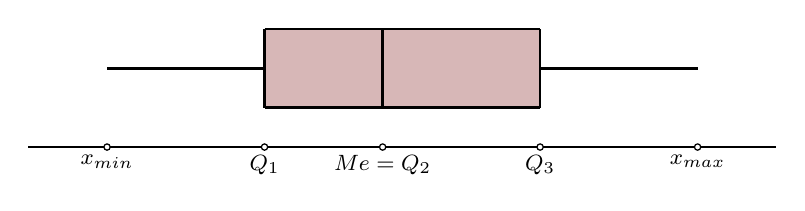
\begin{tikzpicture}
                    % \clip (0,0) rectangle (14.000000,10.000000);
                    {\footnotesize
                    
                    % Marking point x_{min} by circle
                    \draw [line width=0.016cm] (1.500000,1.000000) circle (0.040000);%
                    \draw (1.500000,1.000000) node [anchor=north] { $x_{min}$ };%
                    
                    % Marking point Q_1 by circle
                    \draw [line width=0.016cm] (3.500000,1.000000) circle (0.040000);%
                    \draw (3.500000,1.000000) node [anchor=north] { $Q_1$ };%
                    
                    % Marking point Me=Q_2 by circle
                    \draw [line width=0.016cm] (5.000000,1.000000) circle (0.040000);%
                    \draw (5.000000,1.000000) node [anchor=north] { $Me=Q_2$ };%
                    
                    % Marking point Q_3 by circle
                    \draw [line width=0.016cm] (7.000000,1.000000) circle (0.040000);%
                    \draw (7.000000,1.000000) node [anchor=north] { $Q_3$ };%
                    
                    % Marking point x_{max} by circle
                    \draw [line width=0.016cm] (9.000000,1.000000) circle (0.040000);%
                    \draw (9.000000,1.000000) node [anchor=north] { $x_{max}$ };%
                    
                    % Drawing segment a b
                    \draw [line width=0.016cm] (0.500000,1.000000) -- (1.460000,1.000000);%
                    \draw [line width=0.016cm] (1.540000,1.000000) -- (3.460000,1.000000);%
                    \draw [line width=0.016cm] (3.540000,1.000000) -- (4.960000,1.000000);%
                    \draw [line width=0.016cm] (5.040000,1.000000) -- (6.960000,1.000000);%
                    \draw [line width=0.016cm] (7.040000,1.000000) -- (8.960000,1.000000);%
                    \draw [line width=0.016cm] (9.040000,1.000000) -- (10.000000,1.000000);%
                    
                    % Changing color 215 183 183
                    \definecolor{r215g183b183}{rgb}{0.843137,0.717647,0.717647}%
                    \color{r215g183b183}% 
                    
                    % Filling rectangle left-bottom: f right-top: i
                    \fill (3.500000,2.500000) -- (7.000000,2.500000) -- (7.000000,1.500000) -- (3.500000,1.500000);%
                    
                    % Changing color 0 0 0
                    \definecolor{r0g0b0}{rgb}{0.000000,0.000000,0.000000}%
                    \color{r0g0b0}% 
                    
                    % Drawing segment c d
                    \draw [line width=0.032cm] (1.500000,2.000000) -- (3.500000,2.000000);%
                    
                    % Drawing segment e f
                    \draw [line width=0.032cm] (3.500000,1.500000) -- (3.500000,2.500000);%
                    
                    % Drawing segment g h
                    \draw [line width=0.032cm] (5.000000,1.500000) -- (5.000000,2.500000);%
                    
                    % Drawing segment i j
                    \draw [line width=0.032cm] (7.000000,1.500000) -- (7.000000,2.500000);%
                    
                    % Drawing segment k l
                    \draw [line width=0.032cm] (7.000000,2.000000) -- (9.000000,2.000000);%
                    
                    % Drawing segment e i
                    \draw [line width=0.032cm] (3.500000,1.500000) -- (7.000000,1.500000);%
                    
                    % Drawing segment f j
                    \draw [line width=0.032cm] (3.500000,2.500000) -- (7.000000,2.500000);%
                    \color{black}
                    }
                    \end{tikzpicture}
                \end{figure}
            \end{block}
        \end{frame}


        %%%% naloge

        \begin{frame}
            \only<2->{\begin{exampleblock}{Naloga}
                Izračunajte aritmetično sredino količin.
                \begin{itemize}
                    \item $1.5~s$, $3.5~s$, $1~s$
                    \item $4~km$, $2000~m$, $3~km$
                    \item $4~€$, $2~€$, $3~€$, $1~€$, $5~€$
                \end{itemize}
            \end{exampleblock}}

            \only<3->{\begin{exampleblock}{Naloga}
                Izračunajte aritmetično sredino danim podatkom.
                \begin{itemize}
                    \item $2, 3, 1, 8, 19, 2, 7$
                    \item $13, 39, 12$
                    \item $0.3, 0.4, 0.5, 0.7, 0.6$
                \end{itemize}            \end{exampleblock}}
        \end{frame}

        \begin{frame}
            \only<2->{\begin{exampleblock}{Naloga}
                Določite modus danim številskim podatkom.
                \begin{itemize}
                    \item $1, 4, 2, 4, 1, 6, 3, 4, 1, 4, 6, 4, 4, 8$
                    \item $3, 25, 10, 3, 5, 7, 5, 7, 9, 4, 49$
                    \item $\dfrac{1}{3}, \dfrac{3}{4}, \dfrac{1}{2}, \dfrac{6}{8}, \dfrac{2}{9}$
                    \item $\dfrac{1}{2}, \dfrac{2}{4}, \dfrac{1}{4}, \dfrac{5}{10}, \dfrac{8}{9}$
                \end{itemize}
            \end{exampleblock}}

            \only<3->{\begin{exampleblock}{Naloga}
                V porodnišnici so izmerili dolžine dojenčkov, ki so se rodili v enem dnevu.  \\
                $50, 51, 51, 44, 47, 48, 53, 49, 52, 55, 46, 50, 50, 49, 47, 47$ \\
                Določite mediano podatkov.
            \end{exampleblock}}

        \end{frame}

        \begin{frame}
        
            \only<2->{\begin{exampleblock}{Naloga}
             
             Otroci v vrtcu so metali žogo na koš in si zapisovali dosežke. Podatki so prikazani v preglednici. \\

                 \begin{table}
                     \centering
                     \begin{tabular}{||c|c|c|c|c|c|c|c|c|c||} 
                     \hhline{|t:==========:t|}
                     \rowcolor[rgb]{0.843,0.718,0.718} 
                     Otrok  & Jaka & Jure & Miha & Polona & Valerija & Tina & Mojca & Cene & Darja   \\ 
                     \hhline{|:==========:|}
                     Št.~košev & $5$ & $7$ & $10$ & $8$ & $5$ & $6$ & $9$ & $9$& $4$  \\ 
                     \hhline{|b:==========:b|}
                     \end{tabular}
                 \end{table}

                Izračunajte, koliko košev je otrok zadel v povprečju. Podatke uredite po vrsti in določite $Mo$, $Me$ ter narišite škatlo z brki.

            \end{exampleblock}}

     \end{frame}




    \subsection{Mere razpršenosti}

        \begin{frame}
            \frametitle{Mere razpršenosti}

            \only<2->{\begin{block}{}
                Informacijo o \textbf{porazdelitvi} oziroma \textbf{razpršenosti} podatkov lahko izračunamo s pomočjo: 
                variacijskega razmika, interkvartilnega ranga, variance in standarnega odklona.
            \end{block}}

            \only<3->{\begin{alertblock}{Variacijski razmik}
                \textbf{Variacijski razmik} $R$ je razlika med maksimalno in minimalno vrednostjo statistične spremenljivke:
                $$R=x_{max}-x_{min}.$$
            \end{alertblock}}

            \only<4->{\begin{block}{}
                Variacijski razmik je zelo odvisen od ekstremnih vrednosti, posebno osamelcev, 
                zato ga uporabljamo le v kombinaciji z drugimi merami razpršenosti.
            \end{block}}

        \end{frame}

        \begin{frame}
            \only<2->{\begin{alertblock}{Interkvartilni rang}
                \textbf{Interkvartilni rang} oziroma \textbf{medčetrtinski razmik} $IR$ je razlika med vrednostjo prvega in tretjega kvartila:
                $$IR=Q_3-Q_1.$$
            \end{alertblock}}

            \only<3->{\begin{alertblock}{}
                \textbf{Osamelec} je podatek, katerega vrednost je za več kot $3$-kratnik interkvartilnega ranga~$IR$ nad tretjim kvartilom $Q_3$ ali pod prvim kvartilom $Q_1$. \\
                Podatek je ``pogojno osamelec'', če je njegova vrednost za več kot $1.5$-kratnik interkvartilnega ranga~$IR$ nad tretjim kvartilom $Q_3$ ali pod prvim kvartilom $Q_1$.

            \end{alertblock}}

            \only<4->{\begin{block}{}
                Interkvartilni rang je mera razpršenosti, ki ni občutljiva na osamelce.
            \end{block}}
        \end{frame}

        \begin{frame}

            \only<2->{\begin{alertblock}{Varianca}
                \textbf{Varianca} $\sigma^2$ predstavlja aritmetično sredino kvadratov odmikov vrednosti statistične spremenljivke od aritmetične sredine:
                $$\sigma^2=\dfrac{(x_1-\overline{x})^2+(x_2-\overline{x})^2+\cdots+(x_n-\overline{x})^2}{N}=\dfrac{1}{N}\sum_{i=1}^n(x_i-\overline{x})^2.$$
            \end{alertblock}}

            % \begin{block}{}
            %     Večja kot je varianca, bolj so podatki razpršeni.
            % \end{block}

            \only<3->{\begin{alertblock}{Standardni odklon}
                \textbf{Standardni odklon} $\sigma$ izračunamo kot koren variance:
                $$\sigma=\sqrt{\dfrac{(x_1-\overline{x})^2+(x_2-\overline{x})^2+\cdots+(x_n-\overline{x})^2}{N}}=\sqrt{\dfrac{1}{N}\sum_{i=1}^n(x_i-\overline{x})^2}.$$
                Predstavlja povprečje odmikov vrednosti statistične spremenljivke od aritmetične sredine.
            \end{alertblock}}
        \end{frame}


        %%% naloge

        \begin{frame}
        
            \only<2->{\begin{exampleblock}{Naloga}
             
                V preglednici so predstavljene cene treh izdelkov v trgovini po posameznih mesecih leta 2019. \\
                Izračunajte povprečno ceno in standardni odklon cene vsakega izdelka.

                 \begin{table}
                     \centering
                     \begin{tabular}{||c|c|c|c|c|c|c|c|c|c|c|c||} 
                     \hhline{|t:============:t|}
                     \rowcolor[rgb]{0.843,0.718,0.718} 
                     Izdelek  & Jan & Feb & Mar & Apr & Maj & Jun & Jul & Avg & Sep & Okt & Nov    \\ 
                     \hhline{|:============:|}
                     Kruh  & $3.35$ & $3.29$ & $3.34$ & $3.38$ & $3.38$ & $3.37$ & $3.38$ & $3.55$ & $3.53$ & $3.54$ & $3.49$ \\ 
                     \hhline{|:============:|}
                     Jagode & $8.73$ & $7.18$ & $5.52$ & $4.48$ & $5.72$ & $5.64$ & $6.49$ & $6.58$ & $7.15$ & $7.58$ & $8.34$ \\ 
                     \hhline{|:============:|}
                     Cvetača & $2.04$ & $2.17$ & $1.58$ & $1.75$ & $2.13$ & $1.85$ & $1.93$ & $1.87$ & $1.81$ & $1.99$ & $1.80$ \\ 
                     \hhline{|b:============:b|}
                     \end{tabular}
                 \end{table}
             
                \end{exampleblock}}
 \end{frame}


     \begin{frame}
        
        \only<2->{\begin{exampleblock}{Naloga}
         
            V preglednici je prikazano število rojstev v Sloveniji po letih. \\
            Izračunajte povprečno število rojstev in standardni odklon.

             \begin{table}
                 \centering
                 \begin{tabular}{||c|c|c|c|c|c|c|c|c|c||} 
                 \hhline{|t:==========:t|}
                 \rowcolor[rgb]{0.843,0.718,0.718} 
                 Leto   & $2013$ & $2014$ & $2015$ & $2016$ & $2017$ & $2018$ & $2019$ & $2020$ & $2021$    \\ 
                 \hhline{|:==========:|}
                 Število  & $21111$ & $21165$ & $20641$ & $20345$ & $20241$ & $19585$ & $19328$ & $18767$ & $18989$ \\ 
                 \hhline{|b:==========:b|}
                 \end{tabular}
             \end{table}
        \end{exampleblock}}


             \only<3->{\begin{exampleblock}{Naloga}
         
                Pridobili smo podatke (urejene po velikosti): $1, 13, 14, 15, 15, 15, 17, 18, 18, 19, 19, 19$, $19, 20$ in $40$.
                \begin{itemize}
                    \item Opišite razpršenost podatkov $R$, $IR$, $Q_1$, $Q_3$, $\sigma$, $\overline{x}$.
                    \item Največjo in najmanjšo vrednost (v tem primeru sta to osamelca) odstranimo. Kako se spremeni razpršenost podatkov? 
                \end{itemize}
                
            \end{exampleblock}}
    
         
 \end{frame}



    \subsection{Grafično prikazovanje podatkov}
        
        \begin{frame}
            \frametitle{Grafično prikazovanje podatkov}

            \vskip-1.3em
            \begin{columns}
                \column{0.45\textwidth}
                    \begin{alertblock}{Strukturni krog}
                        \textbf{Strukturni krog} ali \textbf{krožni diagram} uporabljamo, kadar so podatki razvrščeni v malo frekvenčnih razredov 
                        ali ne dosežejo veliko različnih diskretnih vrednosti.
                    \end{alertblock}

                    \begin{block}{}
                        Celoto predstavlja $360^\circ$, za ostale deleže središčne kote izračunamo s sklepnim računom.
                    \end{block}
                \column{0.5\textwidth}            
                \begin{block}{}
                    \begin{figure}[H]
                        \includegraphics[scale=0.25]{../../Slike_in_skice/10921.jpg}
                        \includegraphics[scale=0.25]{../../Slike_in_skice/1092.jpg}
                    \end{figure}
                \end{block}
            \end{columns}

        \end{frame}

        \begin{frame}

            \begin{alertblock}{Stolpčni diagram}
                \textbf{Stolpčni diagram} uporabljamo, ko so podatki razvrščeni v veliko frekvenčnih razredov
                ali lahko dosežejo veliko diskretnih vrednosti.
            \end{alertblock}

            \vskip-1.3em

            \begin{columns}
                \column{0.43\textwidth}

                    \begin{block}{}
                        Stolpčni diagrami so lahko \textbf{pokončni} ali \textbf{ležeči}. 
                        Če želimo prikazati več podatkov naenkrat, uporabimo \textbf{sestavljeni} ali \textbf{strukturni} stolpčni diagram.
                    \end{block}
                \column{0.55\textwidth}            
                \begin{block}{}
                    \begin{figure}[H]
                        \includegraphics[scale=0.28]{../../Slike_in_skice/1093.jpg}
                    \end{figure}
                \end{block}
            \end{columns}
    
        \end{frame}

        \begin{frame}
            \vskip-1.3em

            \begin{columns}
                \column{0.49\textwidth}

            \begin{block}{}
                \begin{figure}[H]
                    \includegraphics[scale=0.19]{../../Slike_in_skice/1095.jpg}
                \end{figure}
            \end{block}

            \column{0.49\textwidth}            
            \begin{block}{}
                \begin{figure}[H]
                    \includegraphics[scale=0.19]{../../Slike_in_skice/1097.jpg} 
                % \end{figure}
            % \end{block}

            % \begin{block}{}
                % \begin{figure}[H]
                    \includegraphics[scale=0.19]{../../Slike_in_skice/1096.jpg}
                \end{figure}
            \end{block}

        \end{columns}

        \end{frame}

        \begin{frame}

                    \begin{alertblock}{Histogram}
                        \textbf{Histogram} uporabljamo za prikaz grupiranih podatkov. 
                    \end{alertblock}

                    \vskip-1.5em
            \begin{columns}
                \column{0.32\textwidth}


                    \begin{block}{}
                        Širine frekvenčnih razredov niso nujno enake.
                        Meje razredov narišemo na vodoravni osi, frekvence posameznih razredov pa na navpični osi.
                    \end{block}
                \column{0.65\textwidth}
                    \begin{block}{}
                        \begin{figure}
                            \includegraphics[scale=0.33]{../../Slike_in_skice/1098.jpg}
                        \end{figure}
                    \end{block}
            \end{columns}


        \end{frame}

        \begin{frame}

            \begin{alertblock}{Linijski diagram}
                \textbf{Linijski diagram/poligon} uporabljamo, ko želimo prikazati postopno spreminjanje vrednosti nekega podatka skozi daljše časovno obdobje.
                Frekvenčne porazdelitve ponazorimo s \textbf{frekvenčnim poligonom}, podatki so lahko zvezni ali grupirani.
            \end{alertblock}

            \vskip-1.3em
            \begin{columns}
                \column{0.58\textwidth}

                    \begin{block}{}
                        \begin{figure}[H]
                            \includegraphics[scale=0.23]{../../Slike_in_skice/1166.jpg}
                        \end{figure}
                    \end{block}

                \column{0.4\textwidth}
                    \begin{block}{}
                        \begin{figure}[H]
                            \includegraphics[scale=0.23]{../../Slike_in_skice/1099.jpg}
                        \end{figure}
                    \end{block}
            \end{columns}

        \end{frame}


        %%%% naloge

        \begin{frame}


            \only<2->{\begin{exampleblock}{Naloga}
         
                Na matematičnem testu je bilo mogoče doseči $50$ točk. Dosežki so bili: 
                $35, 22, 41, 47, 36, 30, 27, 19, 31, 43, 48, 44, 23, 26, 36, 10, 33, 14, 9$. \\
                Razdelite jih v pet enako velikih razredov ter predstavite s histogramom.
                
            \end{exampleblock}}

        
            \only<3->{\begin{exampleblock}{Naloga}
             
             Otroci v vrtcu so metali žogo na koš in si zapisovali dosežke. Podatki so prikazani v preglednici. \\
             Izračunajte, koliko košev je otrok zadel v povprečju. Podatke uredite po vrsti in določite $Mo$, $Me$ ter narišite škatlo z brki.

                 \begin{table}
                     \centering
                     \begin{tabular}{||c|c|c|c|c|c|c|c|c|c||} 
                     \hhline{|t:==========:t|}
                     \rowcolor[rgb]{0.843,0.718,0.718} 
                     Otrok  & Jaka & Jure & Miha & Polona & Valerija & Tina & Mojca & Cene & Darja   \\ 
                     \hhline{|:==========:|}
                     Št.~košev & $5$ & $7$ & $10$ & $8$ & $5$ & $6$ & $9$ & $9$& $4$  \\ 
                     \hhline{|b:==========:b|}
                     \end{tabular}
                 \end{table}
            \end{exampleblock}}

     \end{frame}

     \begin{frame}


   
        \only<2->{\begin{exampleblock}{Naloga}
         
            Bojana beleži, koliko časa potrebuje za pot do šole. Podatke je zapisala v preglednico. \\ 
            S stolpčnim diagramom predstavite, kako pogosto v šolo potuje $8$ minut, $9$ minut ... 

             \begin{table}
                 \centering
                 \begin{tabular}{||c|c|c|c|c|c|c|c|c|c|c||} 
                 \hhline{|t:===========:t|}
                 \rowcolor[rgb]{0.843,0.718,0.718} 
                 Dan  & 1. & 2. & 3. & 4. & 5. & 6. & 7. & 8. & 9. & 10.   \\ 
                 \hhline{|:===========:|}
                 Čas [min] & $9$ & $11$ & $10$ & $8$ & $11$ & $10$ & $9$ & $12$& $9$ & $11$ \\ 
                 \hhline{|b:===========:b|}
                 \end{tabular}
             \end{table}
        \end{exampleblock}}

        \only<3->{\begin{exampleblock}{Naloga}
         
            V domu ostarelih občanov je $500$ oskrbovancev. Od $50$ do $60$ let jih je $15~\%$, med $60$ in $70$ leti je $160$ oskrbovancev,
            med $70$ in $80$ leti pa $200$ starostnikov. Drugi so stari med $80$ in $90$ let.
            \begin{itemize}
                \item Iz grupiranih podatkov izračunajte povprečno starost oskrbovancev tega doma.
                \item Grafično ponazorite starost oskrbovancev.
            \end{itemize}
            
        \end{exampleblock}}


 \end{frame}